\documentclass[onecolumn, draftclsnofoot,10pt, compsoc]{IEEEtran}

\usepackage{graphicx}
\usepackage{url}
\usepackage{setspace}
\usepackage{geometry}
\usepackage{listings}
\usepackage{color}
\usepackage{etoolbox}
\usepackage{pdflscape}

\geometry{textheight=9.5in, textwidth=7in}

% 1. Fill in these details
\def \CapstoneTeamName{			              			 PlanteR-GB}
\def \CapstoneTeamNumber{					           			 Group 64}
\def \GroupMemberOne{				           				Austin Hodgin}
\def \GroupMemberTwo{				           				Travis Hodgin}
\def \GroupMemberThree{			            Maximillian Schmidt}
\def \GroupMemberFour{		        	             Zach Lerew}
\def \CapstoneProjectName{	      	    Winter is Coming...}
\def \CapstoneSponsorCompany{		    Oregon State University}
\def \CapstoneSponsorPerson{		 			  				 Victor Hsu}

% 2. Uncomment the appropriate line below so that the document type works
\def \DocType{		%Problem Statement
				%Requirements Document
				Technology Review
				%Design Document
				%Progress Report
				}

\newcommand{\NameSigPair}[1]{\par
\makebox[2.75in][r]{#1} \hfil 	\makebox[3.25in]{\makebox[2.25in]{\hrulefill} \hfill		\makebox[.75in]{\hrulefill}}
\par\vspace{-12pt} \textit{\tiny\noindent
\makebox[2.75in]{} \hfil		\makebox[3.25in]{\makebox[2.25in][r]{Signature} \hfill	\makebox[.75in][r]{Date}}}}
% 3. If the document is not to be signed, uncomment the RENEWcommand below
\renewcommand{\NameSigPair}[1]{#1}

%%%%%%%%%%%%%%%%%%%%%%%%%%%%%%%%%%%%%%%
\begin{document}
\begin{titlepage}
    \pagenumbering{gobble}
    \begin{singlespace}
    	%\includegraphics[height=4cm]{coe_v_spot1}
        \hfill

        % 4. If you have a logo, use this includegraphics command to put it on the coversheet.
        %
\includegraphics[height=4cm]{derp.jpg}

        \par\vspace{.2in}
        \centering
        \scshape{
            \huge CS Capstone \DocType \par
            {\large\today}\par
            \vspace{.5in}
            \textbf{\Huge\CapstoneProjectName}\par

            %\vfill
						\vspace{1in}

            {\large Prepared for}\par
            \Huge \CapstoneSponsorCompany\par
            \vspace{5pt}
            {\Large\NameSigPair{\CapstoneSponsorPerson}\par}

						\vspace{1in}

            {\large Prepared by}\par
						{\huge \CapstoneTeamNumber}\par
            \CapstoneTeamName\par
            \vspace{5pt}

            {
							\Large
							%\NameSigPair{\GroupMemberOne}\par
							%\NameSigPair{\GroupMemberTwo}\par
							\NameSigPair{\GroupMemberThree}\par
							%\NameSigPair{\GroupMemberFour}\par
            }

            \vspace{20pt}
        }

				\newpage
        \begin{abstract}
				\noindent This is a rough draft. The final draft will have a combined abstract from all team members.
        \end{abstract}
    \end{singlespace}
\end{titlepage}

\newpage

\pagenumbering{arabic}
\tableofcontents
% 7. uncomment this (if applicable). Consider adding a page break.
%\listoffigures
%\listoftables
\clearpage
\singlespace

\newpage


% Syntax highlighting
\definecolor{mygreen}{rgb}{0,0.6,0}
\definecolor{mygray}{rgb}{0.5,0.5,0.5}
\definecolor{mymauve}{rgb}{0.58,0,0.82}

\lstset{
  backgroundcolor=\color{white},   % choose the background color
  basicstyle=\footnotesize,        % size of fonts used for the code
  breaklines=true,                 % automatic line breaking only at whitespace
  captionpos=b,                    % sets the caption-position to bottom
  commentstyle=\color{mygreen},    % comment style
  escapeinside={\%*}{*)},          % if you want to add LTeX within your code
  keywordstyle=\color{blue},       % keyword style
  stringstyle=\color{mymauve},     % string literal style
	frame = single,                  % code framing
}


	% Document body
		%Purpose of tech, derived from tech, example usage, projects that use.
		%Critical thinking, research, comparison to other tech
	\section{Network Interfaces}

		\subsection{Overview and Criteria}
		Version 2.0 of the RGB LED Planter Box begins the with the requirements that a web interface be developed for the controller.
		This web interface will hosted on the local controller (localhost), and only this controller will be accessible to it.
		This is true, only if there isn't a network infrastructure to allow this host to share its web interface to other devices.
	  This network infrastructure must accomodate the web interface host, as well as other clients wishing to interact with the LED array.
		The network must be able to:

		\begin{itemize}
			\item Provide a connection from a client to the web interface host
			\item Be efficient with communications
			\item Easy to implement and manage
		\end{itemize}

		There are many different types of devices and protocols that allow devices to pass information to each other, and share resources.
		Some of these have become more prominent over time due to adaptation and adoption by the majority of industries worldwide.
		Most devices that need to share resources, do so within local limited bounds of an organization.
		Our web interface ideally should be accessible via a LAN or \textbf{L}ocal \textbf{A}rea \textbf{N}etwork.
		LANs connect computers, servers, printers, and embedded devices in a limited space such as a home, school, or office building. \cite{LAN1}
		However, the choice made should leave room to expand, allowing the web interface to be accessible outside the LAN, if the user is able to provide the necessary resources.

		\subsection{Potential Candidates}
		During our research our team has found three commonly used LAN implementations that fit our project's needs.
		The first is a star topology LAN Over Wire, the second is a star topology LAN over wireless radio, and finally a mesh topology LAN over wireless radio.

		\subsection{Star Topology LAN Over Wire}
		Most LANs are based on a star topology.  In this configuration, all end nodes, referred to as clients, are connected to a central hub, which is often a high speed router or switch.
		Each client is connected to the hub via a cable, which is almost always a twisted pair cable.\cite{LAN2}
		In this architecture, all clients are able to communicate to each other by passing their network traffic through the central router.

		\begin{center}
			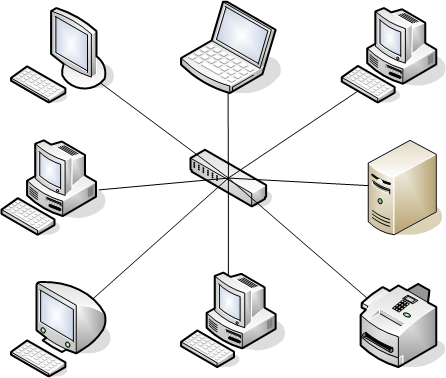
\includegraphics[scale=0.5]{Star_Topology.png}
		\end{center}

		\noindent \\Advantages of using Wire Based Star Topology LANs:
		\begin{itemize}
			\item Traffic sent over wire is guaranteed to reach the destination node, provided the hardware is available.  Having a static physical medium to transfer data across means no data loss.
			\item Connecting new nodes to the network is seamless with IP protocols like DHCP (Dynamic Host Configuration Protocol).
			\item Traffic speed is not inhibited by environmental structure of surrounding area.  As long as the wire connects, one has a constant connection speed.
			\item A single client could fail, but others may continue to communicate on the network due to the architecture.
		\end{itemize}

		\noindent \\Disadvantages of using Wire Based Star Topology LANs:
		\begin{itemize}
			\item The network infrastructure requires a decent amount of hardware.  Each client that wants to connect needs a wire.
			\item Since all traffic is mediated by a central hub:
			\begin{itemize}
				\item If the hub fails, no clients may communicate with each other or the web interface host.
				\item The hub could become a bottleneck for all network resources under heavy traffic.
			\end{itemize}
		\end{itemize}

		\subsection{Star Topology LAN Over Radio}
		This LAN type is nearly the exact same as the wired version, except that clients connect to a hub via wireless radio protocols rather than a cable.
		Standards like IEEE-802.11 allow devices to communicate over radio waves on specific frequencies to pass information to each other.\cite{LAN3}
		Wireless standards have been hammered out just as well as wired standards.

		\noindent \\Advantages of using Wireless Radio Based Star Topology LANs:
		\begin{itemize}
			\item Network infrastructure doesn't require much hardware.  Clients and hub need adapters to communicate via radio waves.
			\item Clients can move around freely, and aren't tied down by fixed length cables.  Cables can also physically get in the way.
		\end{itemize}

		\noindent \\Disadvantages of using Wireless Radio Based Star Topology LANs:
		\begin{itemize}
			\item Wireless radios have to convert wireless signals into understandable frames, and could be slower than wired due to conversion
			\item Radio waves behave like light waves, in that physical objects like walls, can impede the transmission of data.  Data transmission is not guaranteed in every case.
			\item Radios can only handle so many clients transmitting and receiving on a single antennae. Enough clients could slow down a wireless hub.
			\item Disadvantages listed after the first item in \textbf{Star Topology LAN Over Wire}
		\end{itemize}

		%GUI - Front end client makes changes ->
		%GUI - Javascript back end of some sort that takes client requests and reads (parses) config file, writes changes
		%Control service -> Reads changes to config file (parses), update internal state ->
		%Control service -> Applies changes through GPIO or recompile HEX

		\subsection{Mesh Topology LAN Over Radio}
		Similar to the \textbf{Star Topology LAN Over Radio}, clients on this network type use wireless radio transmissions to communicate.
		However, in this network architecture, clients communicate with themselves rather than a central hub, acting as a team to deliver information.
		Clients are aware of their neighbors and the potential routes to deliver information to another client on the network.
		Each node in this network architecture behaves as a router for network traffic.
		A good example would be B.A.T.M.A.N (\textbf{B}etter \textbf{A}pproach \textbf{T}o \textbf{M}obile \textbf{A}d-hoc \textbf{N}etworking).  \cite{LAN4}

		\begin{center}
			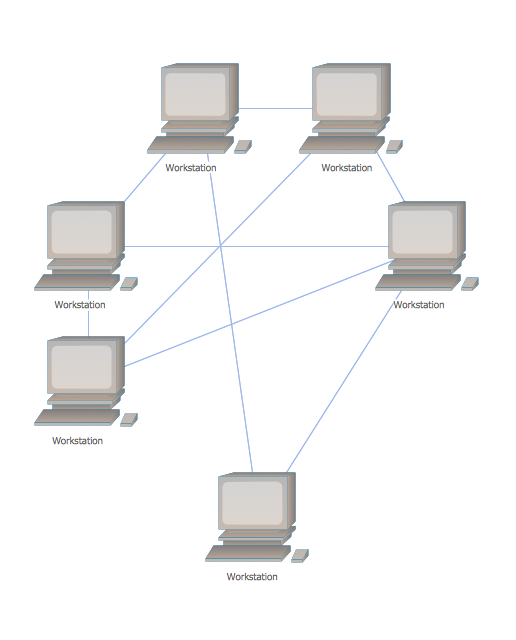
\includegraphics[scale=0.5]{Mesh-network-topology-diagram.png}
		\end{center}

		\noindent \\Advantages of using Mesh Topology LAN Over Radio:
		\begin{itemize}
			\item All advantages listed in \textbf{Star Topology LAN Over Radio}
			\item No single choke point or point of failure in the network
		\end{itemize}

		\noindent \\Disadvantages of using Mesh Topology LAN Over Radio:
		\begin{itemize}
			\item Taking BATMAN for example, it is relatively new and not in wide-spread use.  Further research is needed into implementation.
			\item Set up time is significantly longer than traditional star topology based networks (must be done manually).
			\item Configuring devices to use this network type along side traditional networks can also be a hassle.
		\end{itemize}


		\subsection{Discussion}
		All of these technologies will connect clients to the hosted web interface, but not all of them meet the criteria for simplicity.
		Using a star architecture, one can eliminate any extra setup time, because most devices are already programmed for "plug n' play" on this topology.
		This topology also allows changes to the network to be made easily and quickly.
		This entire network is not going to be extremely complex either.  The project is not aiming for thousands or even hundreds of clients.
		At a maximum, a distributed system in a greenhouse could be comprised of up to 20 controllable beds, each hosting their own interface.
		(This considers a moderate sized greenhouse found at common private nurseries that sell to the public.) 	The project has envisioned multiple levels of systems,
		but none of these levels cannot be achieved by the simplest of the three network types.  All three could handle every requirement, except simplisity in some cases.

		\subsection{Conclusion}
		Due to the need for simplicity of setup, a star type topology is going to be the network architecture used.
		Because most network infrastructure devices can integrate both wired and wireless device, the end network may see a mix of wireless and wired clients.
		For iteration beginnings and the need for even further simplicity to develop on, the team will most likely start with wired connections.



	\section{Custom Enclosure Design}

		\subsection{Overview and Criteria}
		% Add stuffs

		\subsection{3D Printed Hardware}
		% Add stuffs
		\noindent \\Advantages of 3D printing parts for a planter bed:
		\begin{itemize}
			\item Relatively inexpensive compared to other methods or purchasing hardware
			\item If source files provided, 3D printing allows end users to customize the hardware if necessary
			\item Could potentially be quicker to print ones own custom parts, rather than custom order them
		\end{itemize}

		\noindent \\Disadvantages of 3D printing parts for a planter bed:
		\begin{itemize}
			\item The client might have to learn how to use a 3D printer and 3D modeler, adding complexity.
			\item Hardware may not be printed correctly or could be not as strong as something professionally manufactured.
			\item Hardware may take some a long time to print, depending on what is printed
		\end{itemize}


		\subsection{Pre-Fabricated}
		% Add stuffs

		\noindent \\Advantages of Pre-Fabricating Parts:
		\begin{itemize}
			\item Client sets up the beds with a simple guide
			\item Client doesn't have to wait on parts to be made
			\item Client doesn't have to make their own parts
		\end{itemize}

		\noindent \\Disadvantages of Pre-Fabricating Parts:
		\begin{itemize}
			\item Client may not be able to customize the parts to a custom enclosure of their own
			\item Client could end up paying more than other methods
			\item Adds another design implementation to the \textit{software developer's} list (team does not consist of any machinists or mechanical engineers)
		\end{itemize}


		\subsection{"Slap On"-type Connections}
		% Add stuffs

		\noindent \\Advantages of "Slap On"-type Connections:
		\begin{itemize}
			\item The least expensive option provided.  Easy to get replacements.
			\item The easiest to assemble and disassemble makes this option stand out for mobility purposes.
		\end{itemize}

		\noindent \\Disadvantages of "Slap On"-type Connections:
		\begin{itemize}
			\item "You get what you pay for." Items are not durable.
			\item Connections may not hold permanently or are insecure.  Electrical connections might suffer at this option.
			\item Connections may not hold at all, and planter beds may fall apart.
		\end{itemize}


		\subsection{Discussion}
		% Add lots o' stuffs

		\subsection{Conclusion}
		% Add stuffs



		\section{Control Service Language}

			\subsection{Overview and Criteria}
			% Add stuffs

			\subsection{C/C++}
			% Add stuffs

			\noindent \\Advantages of using C/C++:
			%\begin{itemize}
				% Add stuffs
			%\end{itemize}

			\noindent \\Disadvantages of using C/C++:
			%\begin{itemize}
				% Add stuffs
			%\end{itemize}


			\subsection{Web Based Language(NodeJS, PHP, etc)}

			\noindent \\Advantages of using Web Based Language:
			%\begin{itemize}
				% Add stuffs
			%\end{itemize}

			\noindent \\Disadvantages of using Web Based Language:
			%\begin{itemize}
				% Add stuffs
			%\end{itemize}


			\subsection{Rust}
			% Add stuffs

			\noindent \\Advantages of using Rust:
			%\begin{itemize}
				% Add stuffs
			%\end{itemize}

			\noindent \\Disadvantages of using Rust:
			%\begin{itemize}
				% Add stuffs
			%\end{itemize}


			\subsection{Discussion}
			% Add stuffs

			\subsection{Conclusion}
			% Add stuffs


		%References
		\bibliography{ref}
		\bibliographystyle{IEEEtran}

\end{document}
